\chapter{The Atmospheric Emission Model}

Ground-based experiments have been playing and will continue to play a
prominent role in the observation of the cosmic microwave background
radiation temperature and polarisation anisotropies. As compared to
their space-borne or balloon-borne counterparts, ground-based experiments
can deploy larger primary reflectors, achieving higher angular resolution.
However, these instruments must deal with atmospheric effects.

The atmospheric radiation is almost unpolarized, therefore it does not
contribute directly to the signal acquired by instrumentation designed to
measure polarized sources, like the coherent polarimeters of the Strip
telescope. However, residual atmospheric emission inevitably increases the
optical power incident on the detectors and therefore their noise level. In
addition, temporal variations in emission, caused by variable water vapour
content, contribute low frequency correlated noise to the signal.

\section{Atmospheric Radiative Transfer}

The atmosphere can be viewed as a dielectric medium, whose effects on the
incoming electromagnetic radiation are charactherized by the complex permittivity

\begin{equation}
        \epsilon\qty(\nu) = \epsilon_r\qty(\nu) + i\epsilon_i\qty(\nu)
\end{equation}

where $\nu$ is the frequency of the incoming and radiation the real and
imaginary parts, $\epsilon_r$ and $\epsilon_i$ are linked by the
Kramers-Kronig relations

\begin{align}
        \epsilon_r\qty(s) & = \frac{1}{\pi}
        \principalvalue{\int^\infty_{-\infty}\dd{s'}
        \frac{\epsilon_i\qty(s)}{s' - s}} \label{eq:kk_relations_1} \\
        \epsilon_i\qty(s) & = -\frac{1}{\pi}
        \principalvalue{\int^\infty_{-\infty}\dd{s'}
        \frac{\epsilon_r\qty(s)}{s' - s}} \label{eq:kk_relations_2}.
\end{align}

The variable $s = \sigma + i 2\pi\nu$ is the complex frequency and $\sigma$
is the \emph{Neper frequency}.

As is shown in \autoref{fig:transmittance_teide}, contributions to the
atmospheric complex permittivity arise principally from
oxigen and water vapour molecules. Water vapour is responsible for most of
the continuum absorption in the \SIrange{400}{500}{\giga\hertz} frequency
range. The broad absorption oxigen band around \SI{60}{\giga\hertz} and the
oxigen line at \SI{119}{\giga\hertz} contribute to very strong absorption,
as the water vapour lines at \SIlist{22;183;325;380}{\giga\hertz} do. We will
show that the most problematic features of the atmospheric absorption spectrum
regarding the Q-band channels of the Strip telescope are in fact the
\SI{22}{\giga\hertz} water vapour line and the \SI{\sim 60}{\giga\hertz}
oxigen plateau.

\begin{figure}
        \centering
        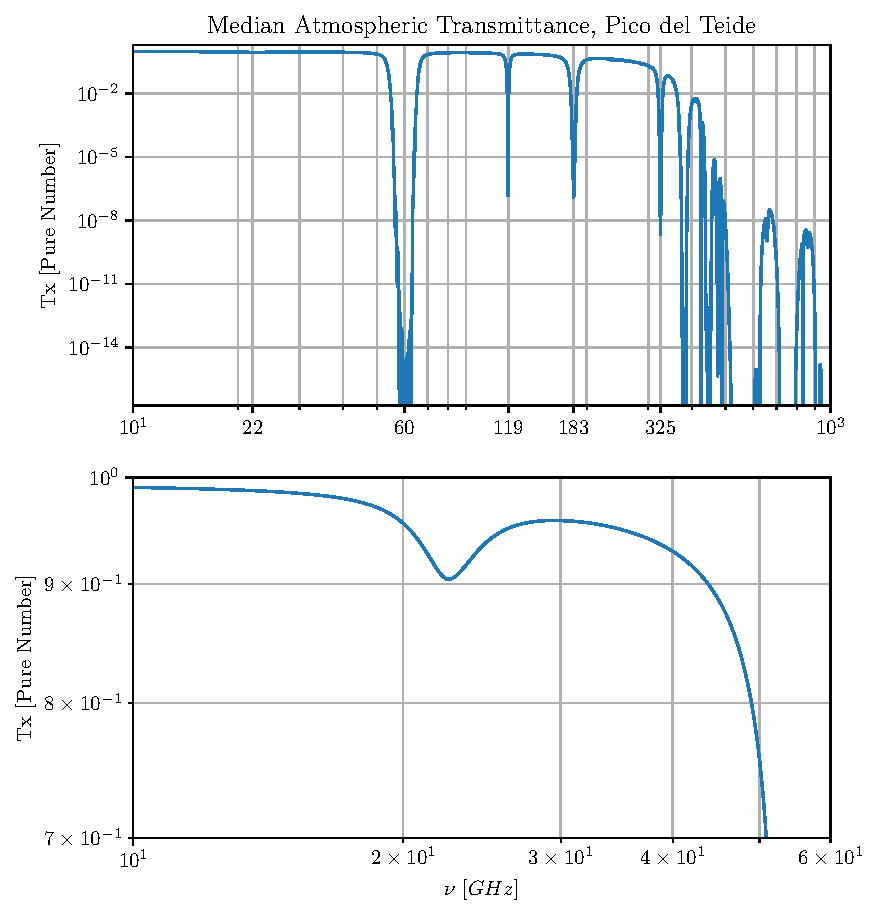
\includegraphics[width=\textwidth]{transmittance_Teide}
        \caption{Atmospheric transmittance at Pico del Teide and low
        frequencies detail. CAL software.}
        \label{fig:transmittance_teide}
\end{figure}


The real and imaginary parts of $\epsilon$ are related to the atmopshere
refractive index, $n\qty(\nu)$, and absorption coefficient, $\alpha\qty(\nu)$,

\begin{align}
        \epsilon_r\qty(\nu) & = \sqrt{n\qty(\nu)} \\
        \epsilon_i\qty(\nu) & = \frac{\lambda \alpha\qty(\nu)}{4\pi}
\end{align}

where $\lambda$ is the wavelength of the incoming radiation.

From \autoref{eq:kk_relations_1} and \autoref{eq:kk_relations_2} follows that
the refractive index and the absorption coefficient are note independent
quantities.

the context of this thesis to obtain estimates for atmospheric brightness
temperatures.

\section{Atmospheric Spatial Structures}
